In this section we shall know about the properties of gravitational waves. Gravitational waves can be characterised by its frequency, amplitude, period. The propagate with the same speed of Electromagnetic waves. Unlike Electromagnetic waves, the wavelength of GW’s can range from a kilometer to the size of the universe itself. Since the wavelength of gravitational waves is larger than the source, they cannot be used for imaging. In contrast to electromagnetic waves which are polarised at 90 degree, i.e orthogonal plane polarized EM waves have their plane 90 degrees apart, where as for gravitational waves it is at 45 degree which will be discussed in the next session. GWs do not interact with matter, but electromagnetic waves do. Electromagnetic waves are known to exhibit a wave-particle duality nature unlike Gravitational waves, the nature of which is still unknown. Although there are quite a few similarities between these two, gravitational waves open a new different window to view the universe. \cite{Thorne:1995xs}

\begin{figure}[h]
    \centering
    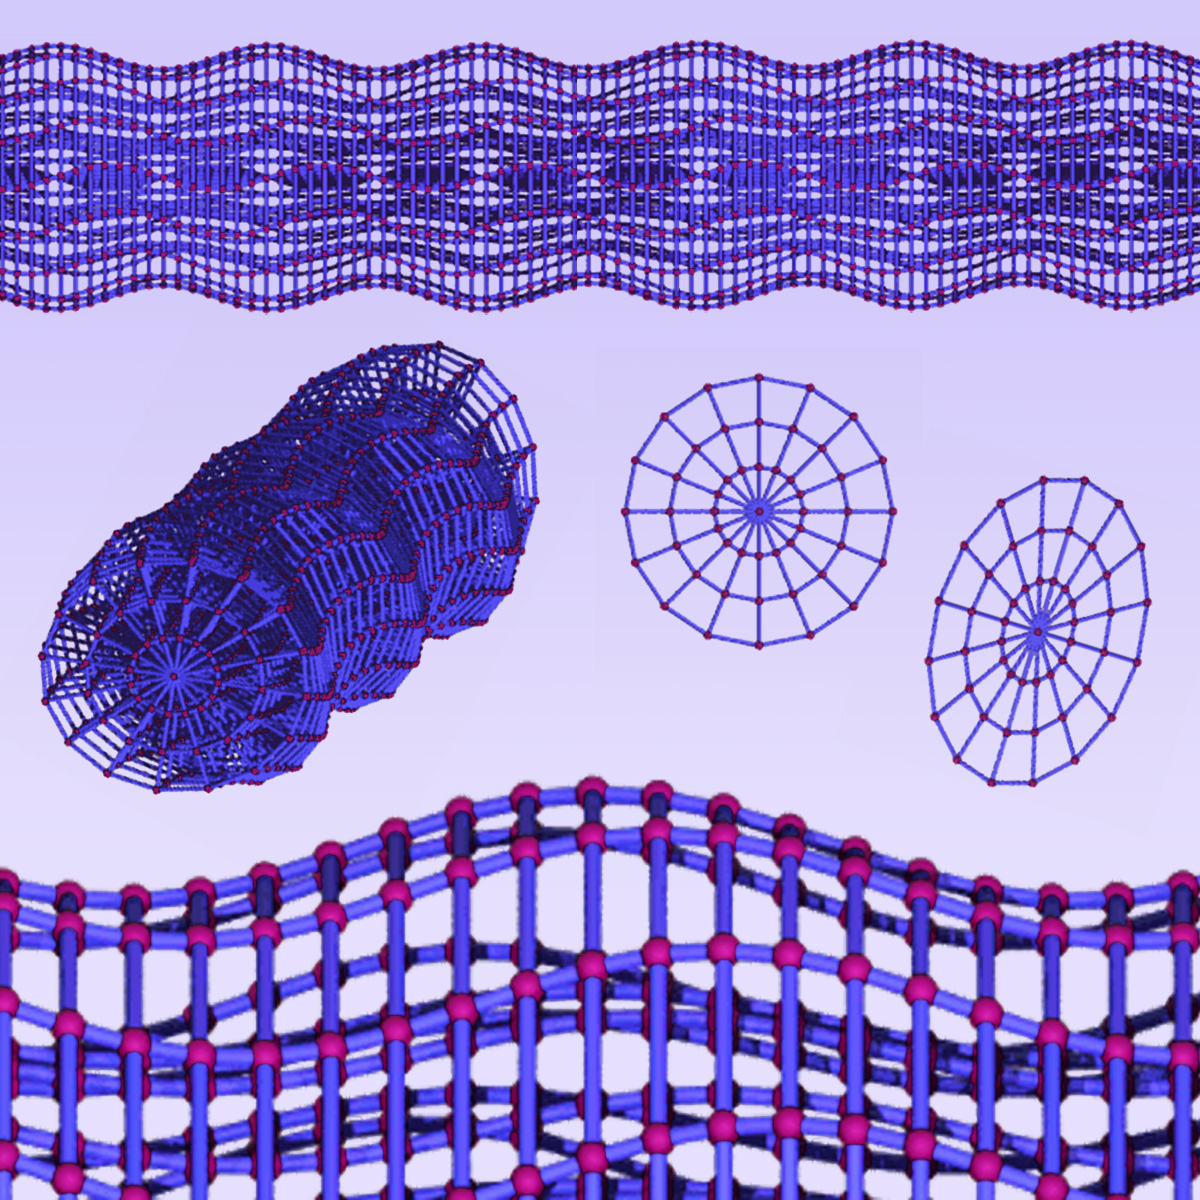
\includegraphics[height= 7cm, width=9cm]{images.tex/GW_propagation.jpg}
    \caption{Propagation of GW wave\\ Source:- \url{https://www.einstein-online.info/en/spotlights/gravwav/gravwav-sub01/}}
\end{figure}

\begin{figure}[h]
    \centering
    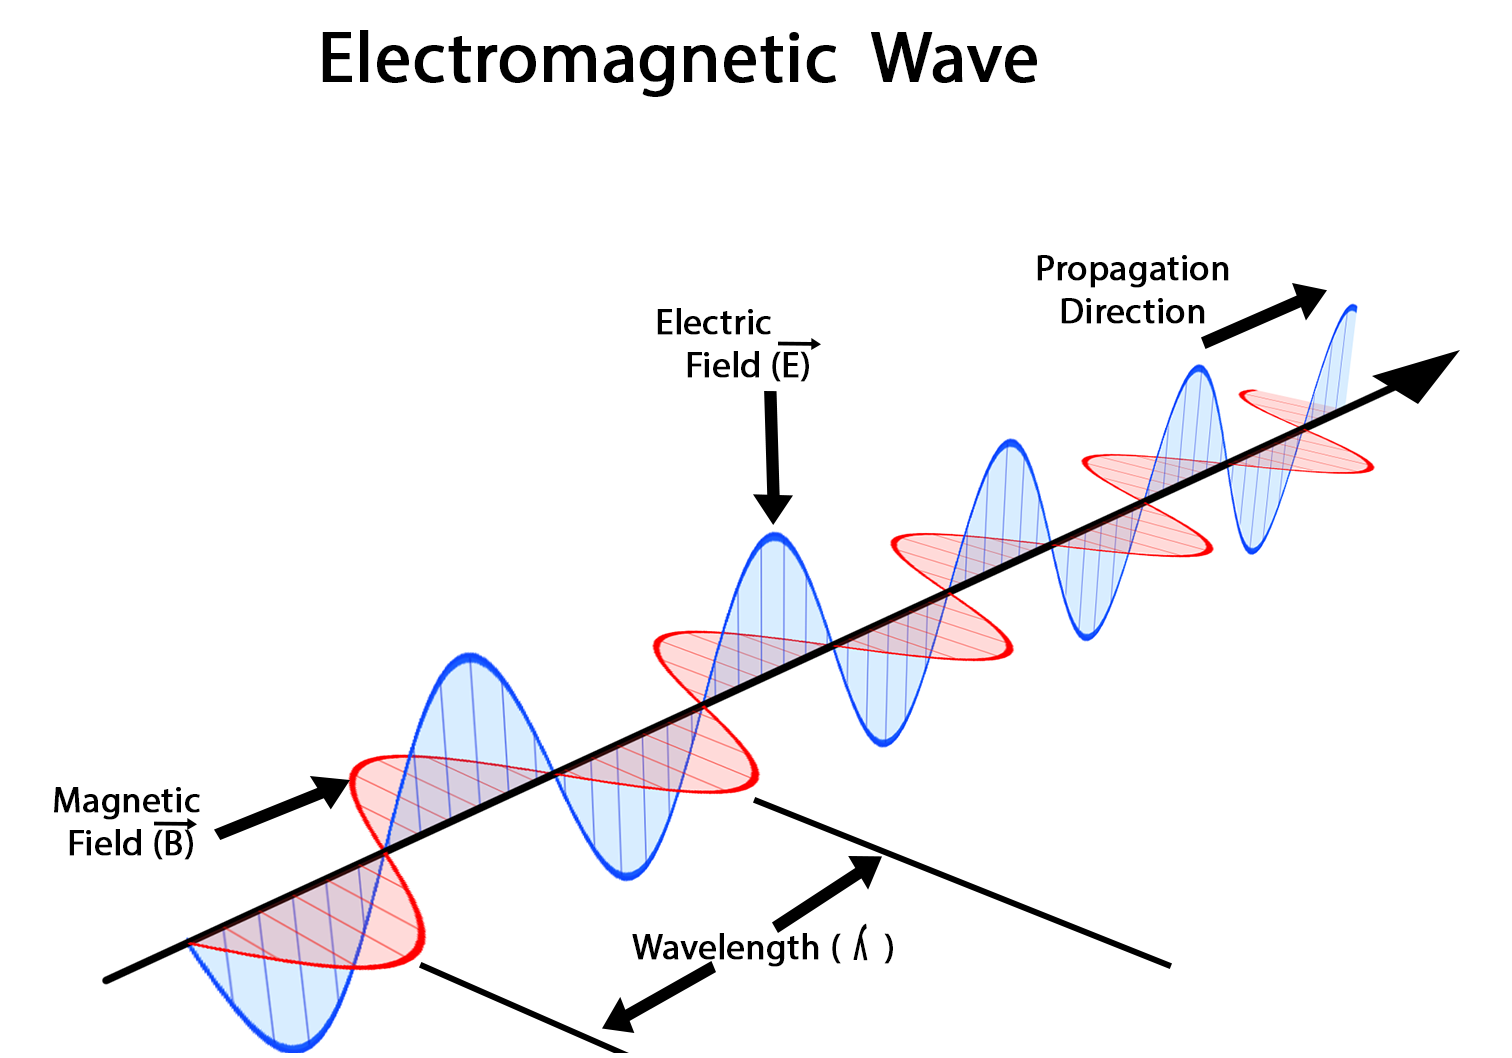
\includegraphics[height= 7cm, width=9cm]{images.tex/EM_propagation.png}
    \caption{Propagation of EM wave\\
    Source:-\;\url{https://www.toppr.com/guides/physics/communication-systems/propagation-of-electromagnetic-waves/}}
\end{figure}

\pagebreak
